\documentclass{beamer}

\usepackage{beamerthemesplit}

\usepackage{xmpmulti}
\usepackage{animate}
\usepackage{amsmath}
\usepackage{physics}
\usepackage{xcolor}
\usepackage{graphicx}
\usepackage{fontawesome5}
\usepackage{tcolorbox}

\usepackage{amssymb}
\usepackage{multirow}
\usepackage{mathtools}

\usepackage{physics}
\usepackage{mathrsfs}

\usepackage{tikz}
\usetikzlibrary{calc}

\usetheme{Copenhagen}
\useoutertheme{infolines}

\newcommand{\iu}{{i\mkern1mu}}

\title[Wobbling Motion]{New Data on Wobbling Motion for A\texorpdfstring{$\approx$}{=}130 Mass Region}

\author[Robert Poenaru]{Robert Poenaru\texorpdfstring{$^{1,2}$}{(1,2)}}

\institute[IFIN-HH]{\texorpdfstring{$^{1}$}{1}Doctoral School of Physics, UB \\ \texorpdfstring{$^{2}$}{2}Department of Theoretical Physics, IFIN-HH}

\date[\today]{\today} % Presentation date or conference/meeting name, the optional parameter can contain a shortened version to appear on the bottom of every slide, while the required parameter value is output to the title slide

\setbeamertemplate{navigation symbols}{}

%%%%%%%%%%%%%%%%%%%%%%%%%%%%%%%%%%%%%
%%%%%%% start of the document %%%%%%%
%%%%%%%%%%%%%%%%%%%%%%%%%%%%%%%%%%%%%

\begin{document}

{\setbeamertemplate{headline}{}
\begin{frame}
	\titlepage
\end{frame}}

\begin{frame}{Outline}
    \tableofcontents
\end{frame} 

\section{Nuclear Triaxiality}


\begin{frame}
	\frametitle{Nuclear Deformation}
	\begin{exampleblock}{Nuclear shapes}
		Most generally described in terms of the \textbf{nuclear radius}:
		\begin{align}
			R(\theta,\varphi)=R_0\left(1+\sum_{\lambda=0}^{^\infty}\sum_{\mu=-\lambda}^\lambda\alpha_{\lambda\mu}Y_\lambda^\mu(\theta,\varphi)\right)\nonumber
		\end{align}
	\end{exampleblock}
	\begin{block}{Quadrupole deformations $\lambda=2$}
		\begin{itemize}
			\item Most relevant modes are the \textbf{quadrupole vibrations} $\lambda=2$ $\Longrightarrow$ \emph{Play a crucial role in the rotational spectra of nuclei:}
			\item $\alpha_{2\mu}$ reduced to only two \emph{deformation parameters}: $\beta_2$ (\textbf{eccentricity}) and $\gamma$ (\textbf{triaxiality}) (\textit{Bohr and Mottelson, 1969}).
		\end{itemize}
	\end{block}
\end{frame}

\begin{frame}
	\frametitle{Axial shapes}
	\vspace{-0.2cm}
	\begin{itemize}
		\item Most of the nuclei are either \textbf{spherical} or \textbf{axially symmetric} in their ground-state. % \textit{(Budaca, 2018)}.
		\item Nuclear moments of inertia $\mathcal{I}_{1,2,3}$: only two are equal.
	\end{itemize}
	\vspace{-0.4cm}
	\begin{figure}
		\centering
		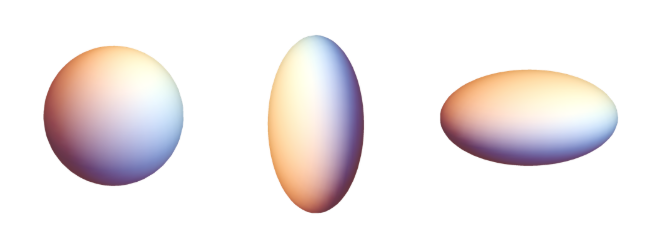
\includegraphics[scale=0.38]{figures/nuclear_shapes.png}
		\caption{\textbf{spherical:} $\beta_2=0$\ \textbf{prolate:} $\beta_2>0$\ \textbf{oblate:} $\beta_2<0$.\ ($\gamma=0^\circ$).}
	\end{figure}
\end{frame}

\begin{frame}
	\frametitle{Non-axial shapes}
	\vspace{-0.2cm}
	\begin{itemize}
		\item The triaxiality parameter $\gamma\neq 0^\circ$: departure from axial symmetry.
		\item Moments of inertia: $\mathcal{I}_{1}\neq\mathcal{I}_{2}\neq\mathcal{I}_{3}$.
	\end{itemize}
	\vspace{-0.2cm}
	\begin{figure}
		\centering
		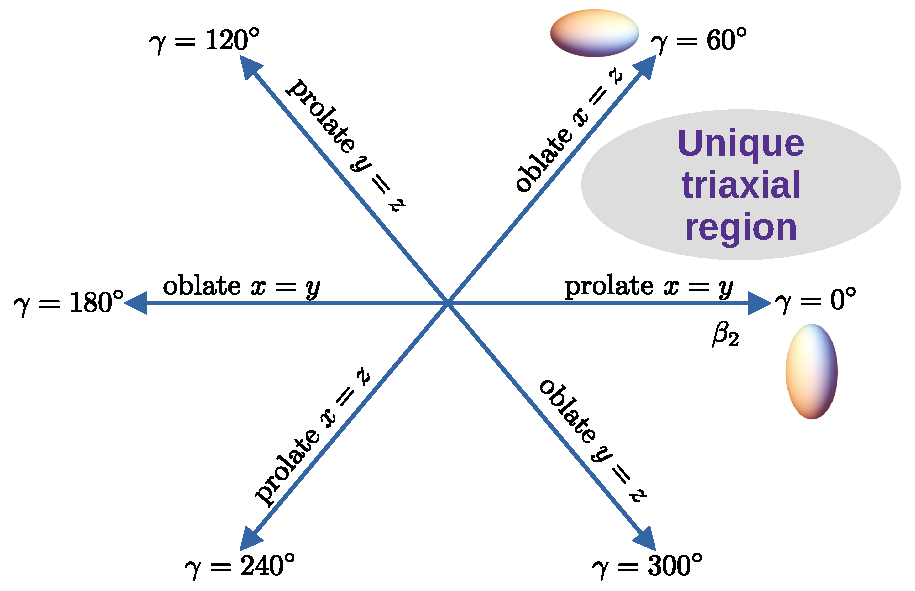
\includegraphics[scale=0.49]{figures/nice_diagram.pdf}
		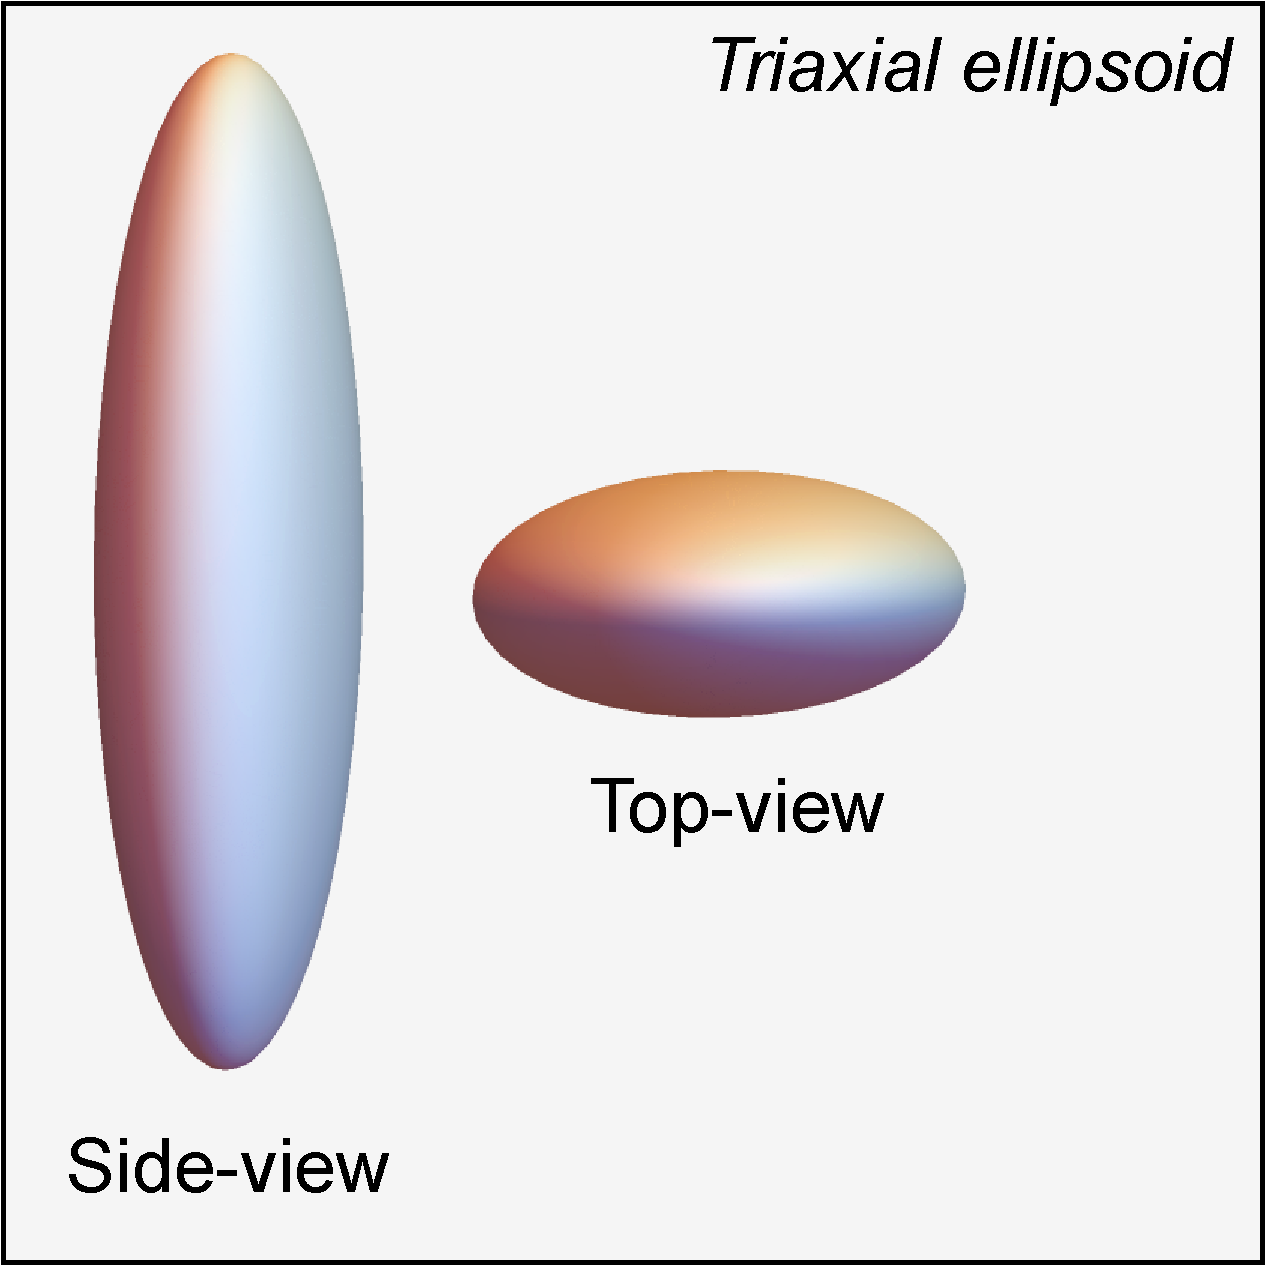
\includegraphics[scale=0.20]{figures/triaxial-shape.pdf}
		\vspace{-0.41cm}
	\end{figure}
\end{frame}

\section{Wobbling Motion in Nuclei}

\begin{frame}
	\frametitle{Wobbling Motion}
	\vspace{-0.4cm}
	\begin{columns}
		\begin{column}{0.55\textwidth}
			\begin{center}
				\begin{tikzpicture}[node distance=1.5cm]
					\node[draw, fill=blue!20!white, text width=3cm, text centered, minimum height=1cm] (box1) {$\gamma\neq0^\circ$};
					\node[draw, fill=blue!20!white, text width=4cm, text centered, minimum height=1cm, below of=box1] (box2) {MOI anisotropy};
					\node[draw, fill=blue!20!white, text width=6cm, text centered, minimum height=1cm, below of=box2] (box3) {\emph{main rotation} around $\mathcal{J}_\text{max}$ is disturbed by the other two axes};
					\draw[->] (box1) -- (box2);
					\draw[->] (box2) -- (box3);
				\end{tikzpicture}
			\end{center}
		\end{column}
		\begin{column}{0.45\textwidth}
			\begin{figure}
				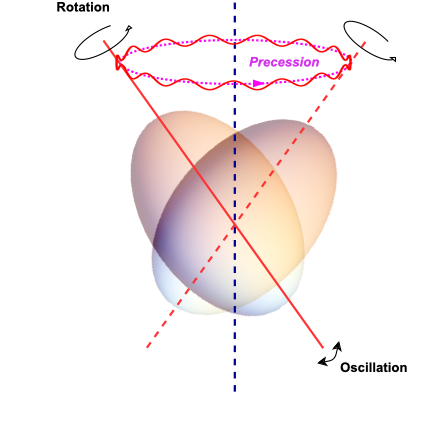
\includegraphics[width=\textwidth]{figures/wobbling-schematic.png}
			\end{figure}
		\end{column}
	\end{columns}
	\vspace{-0.4cm}
	\begin{alertblock}{Wobbling Effect}
		\begin{itemize}
			\item The \textbf{total angular momentum} of the nucleus \textbf{precesses} and \textbf{oscillates} around $\mathcal{J}_\text{max}$.
		\end{itemize}
	\end{alertblock}
\end{frame}


\begin{frame}
	\frametitle{Wobbling Motion}
	\begin{exampleblock}{Harmonic oscillation}
		\begin{itemize}
			\item Precession of $\mathbf{I}$ is affected by \textbf{rotational frequency} and/or \textbf{tilting}
			\item Tilting only by "specific" amount $\rightarrow$ \textbf{harmonic character} $\rightarrow$ \textbf{wobbling phonon}: $n_w=0,1,2,\dots$.
		\end{itemize}
	\end{exampleblock}
	\begin{figure}
		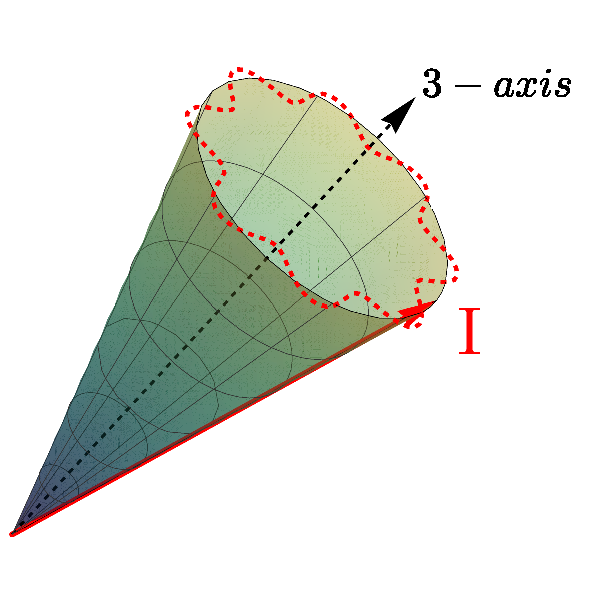
\includegraphics[width=0.32\textwidth]{figures/precessional_cone_2.pdf}
		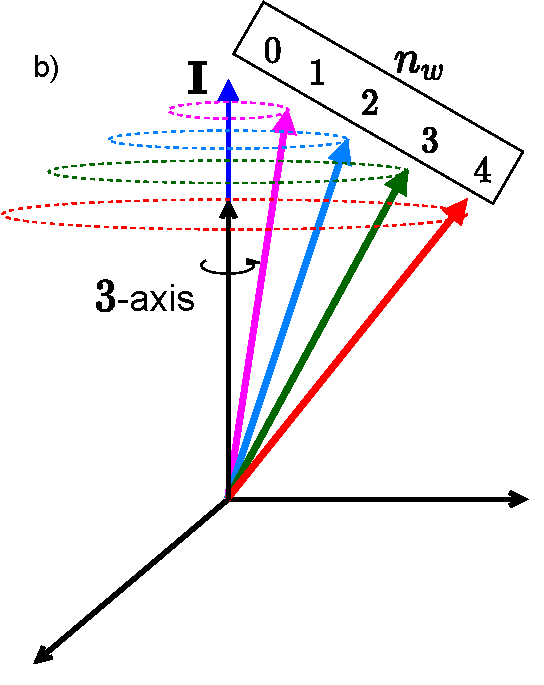
\includegraphics[width=0.3\textwidth]{figures/wobbling_n_schematic-2.pdf}
		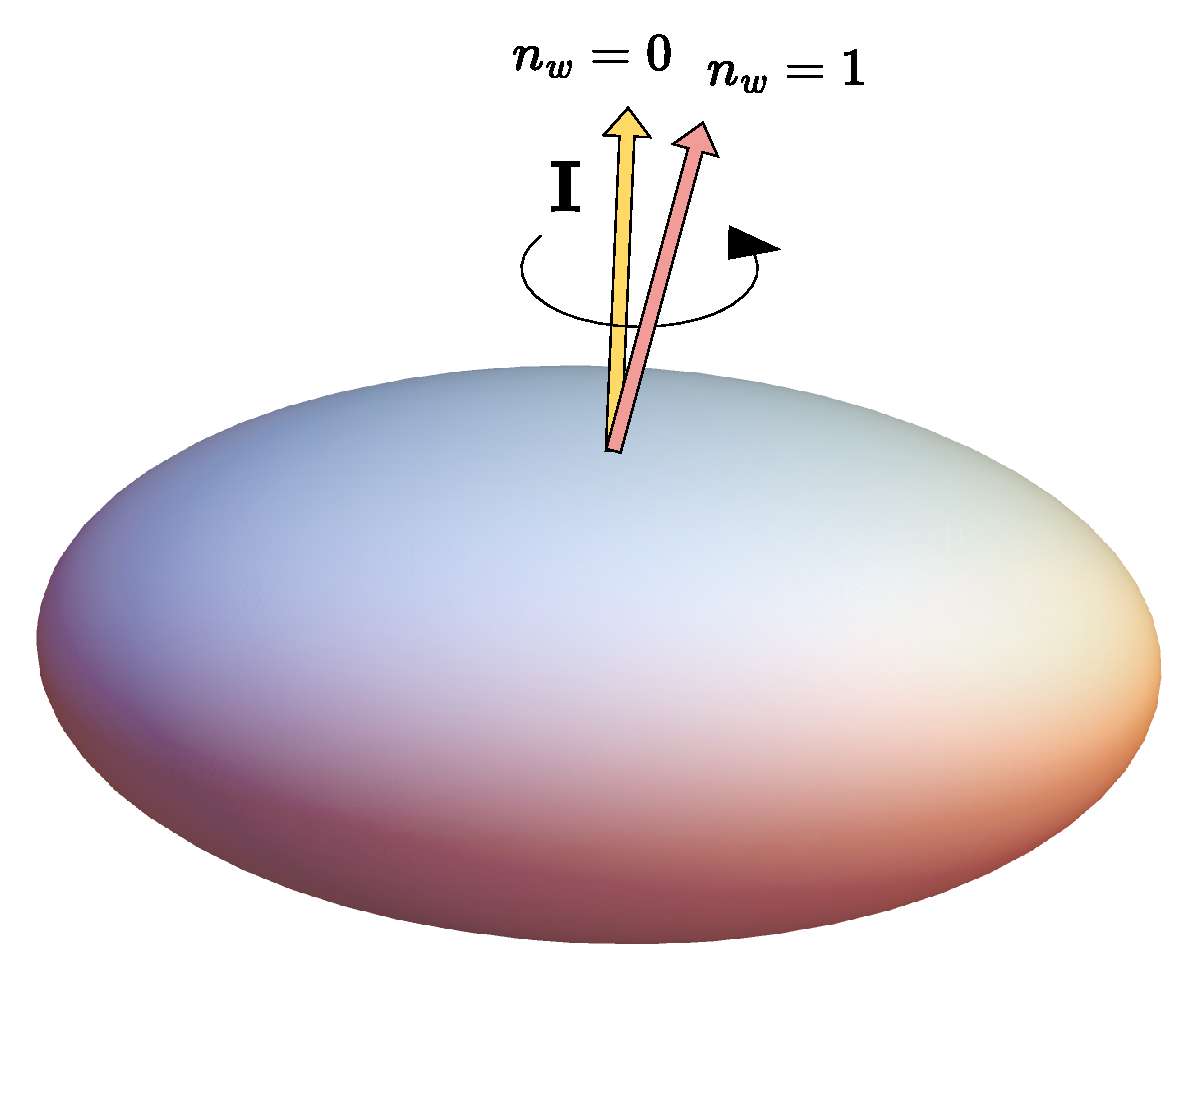
\includegraphics[width=0.34\textwidth]{figures/triaxial-shapes-even-A.pdf}
	\end{figure}
\end{frame}

\begin{frame}
	\frametitle{Wobbling Motion II}
	\vspace{-0.4cm}
	\begin{columns}
		\begin{column}{0.6\textwidth}
			\begin{figure}
				\centering
				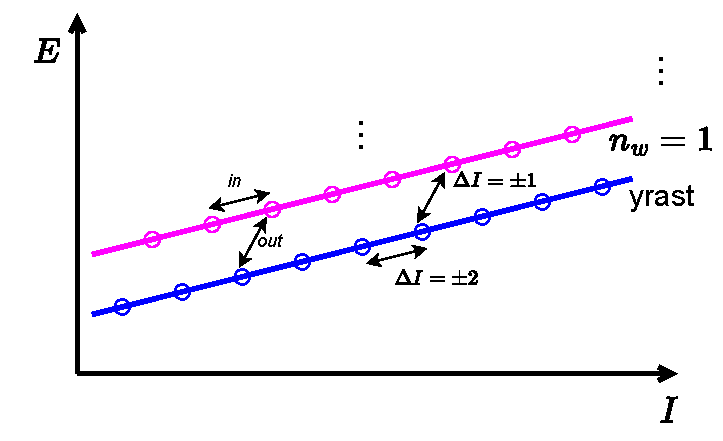
\includegraphics[scale=0.45]{figures/wobbling_n_schematic.drawio.pdf}
				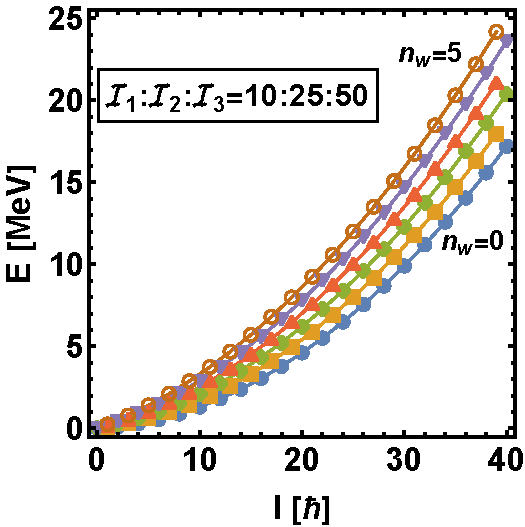
\includegraphics[scale=0.48]{figures/wobblingFreq-evenA.pdf}
			\end{figure}
		\end{column}
		\begin{column}{0.4\textwidth}
			\begin{figure}
				\centering
				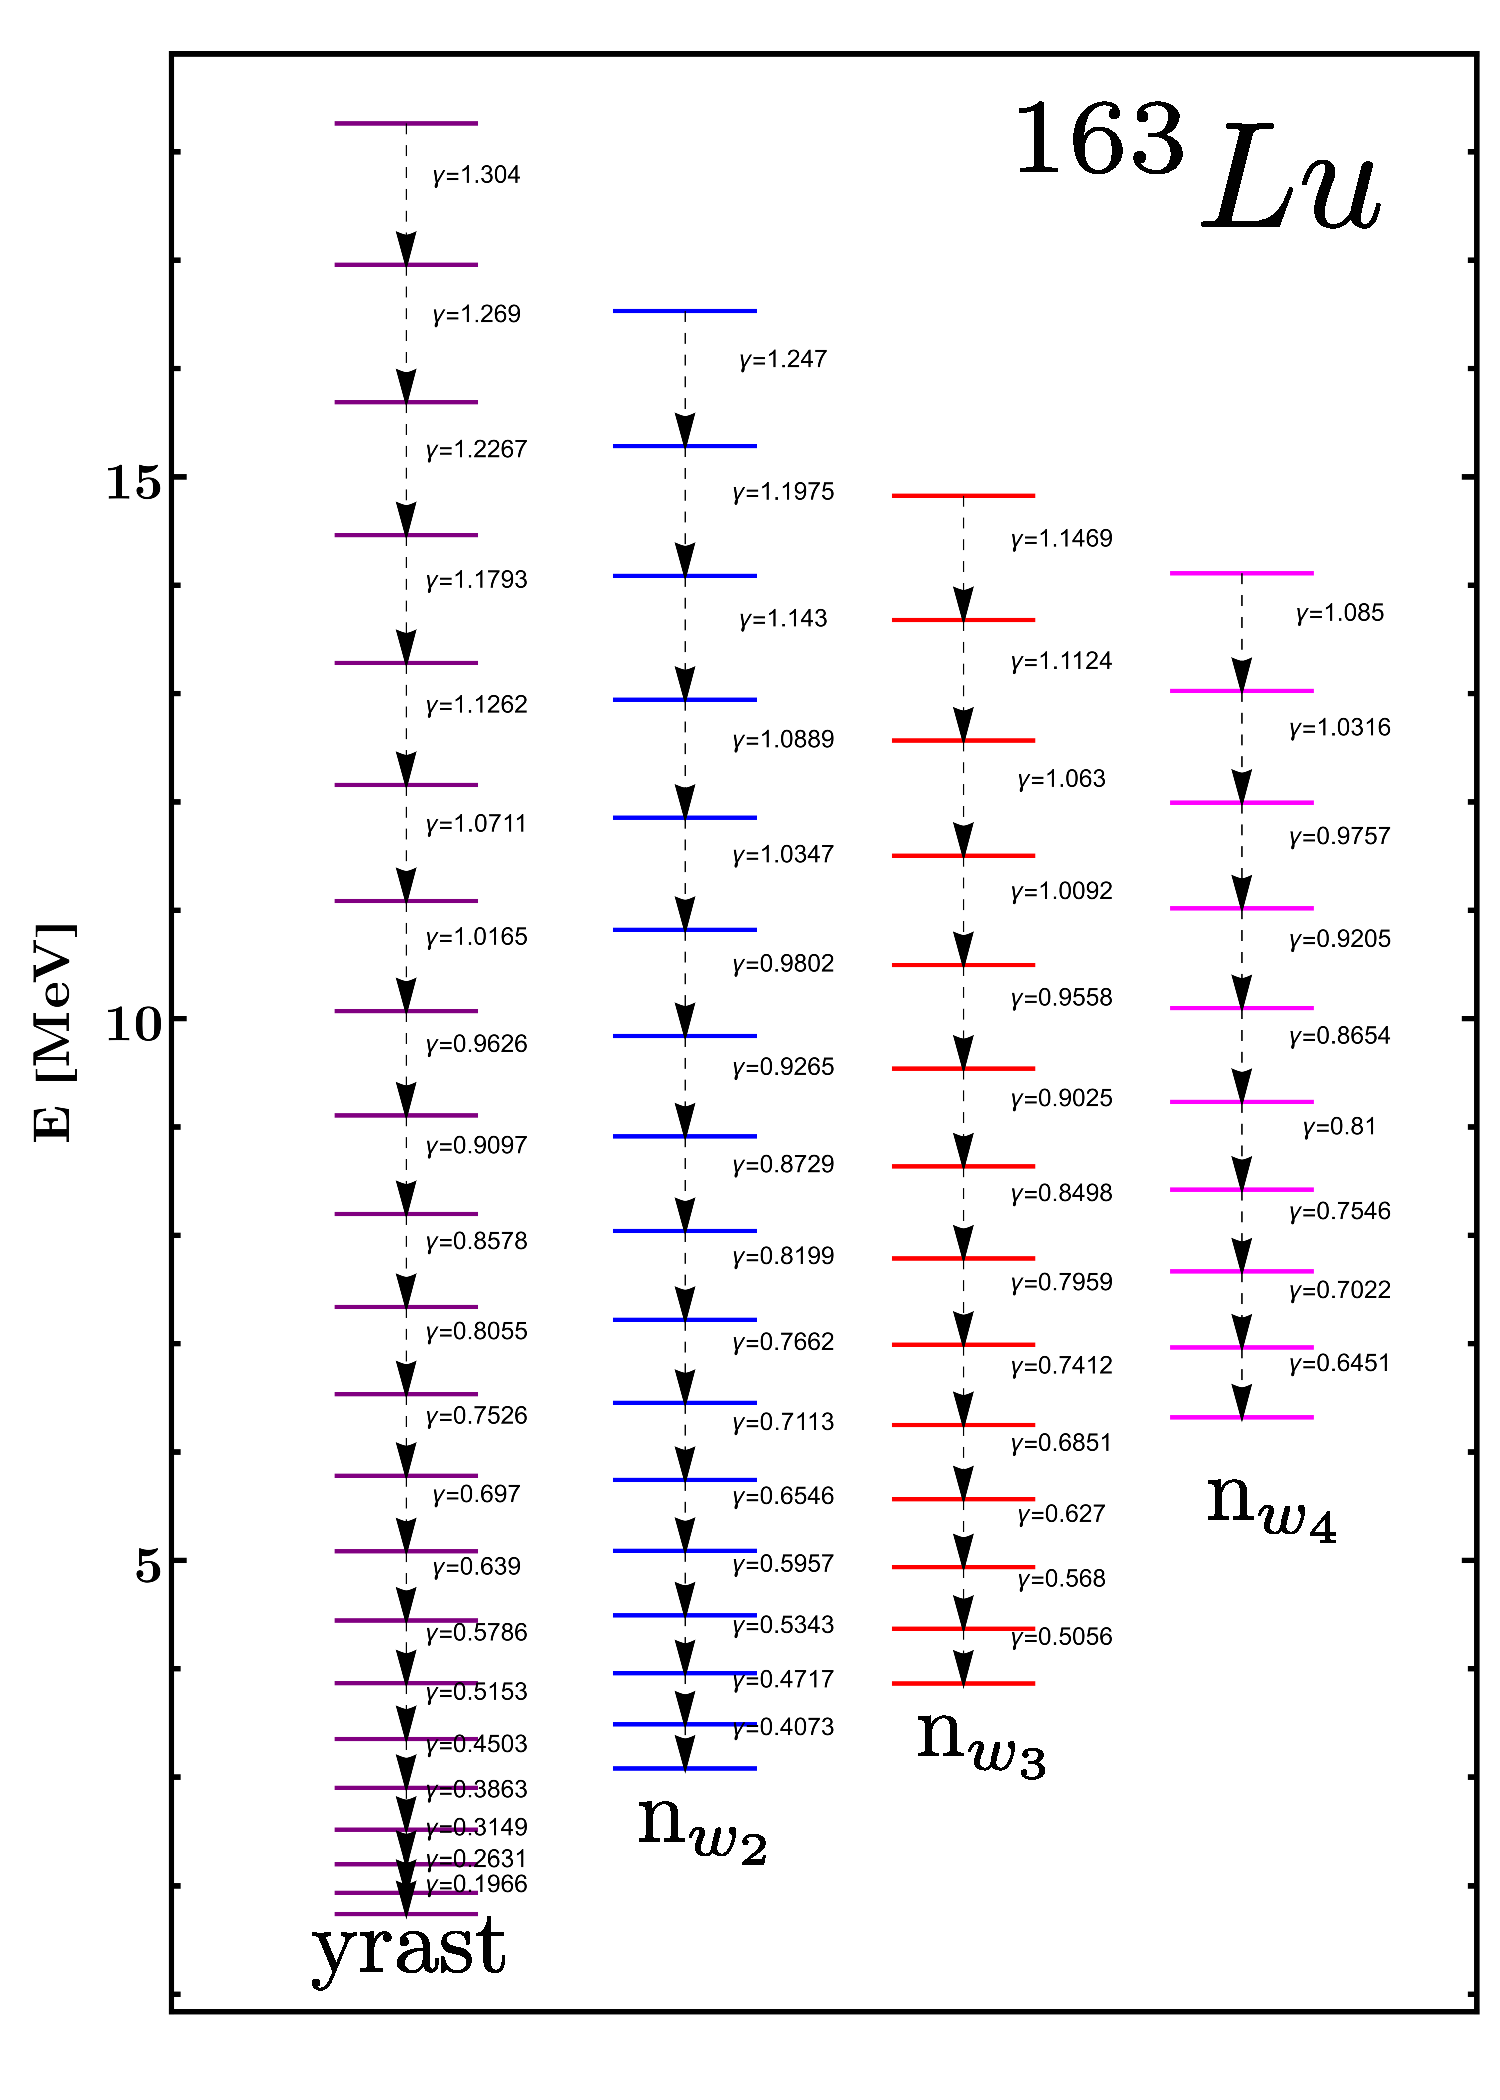
\includegraphics[width=0.99\textwidth]{figures/lu-163-exp-data-eps-converted-to.pdf}
			\end{figure}
			\vspace{-0.4cm}
			\textit{R. Poenaru, 2023}.
		\end{column}
	\end{columns}
\end{frame}

\begin{frame}
	\frametitle{Even-$A$ vs. Odd-$A$ Picture}
	\begin{itemize}
		\item Predicted for even-$A$ nuclei more than 50 years ago.
		\item First experimental evidence: $^{163}$Lu (\textit{Ødegård, 2001}). %  for \textbf{nuclear wobbling motion}
		\item Current mass-regions for wobblers: $A\approx[130,160,180]$.
	\end{itemize}
	\begin{figure}
		\centering
		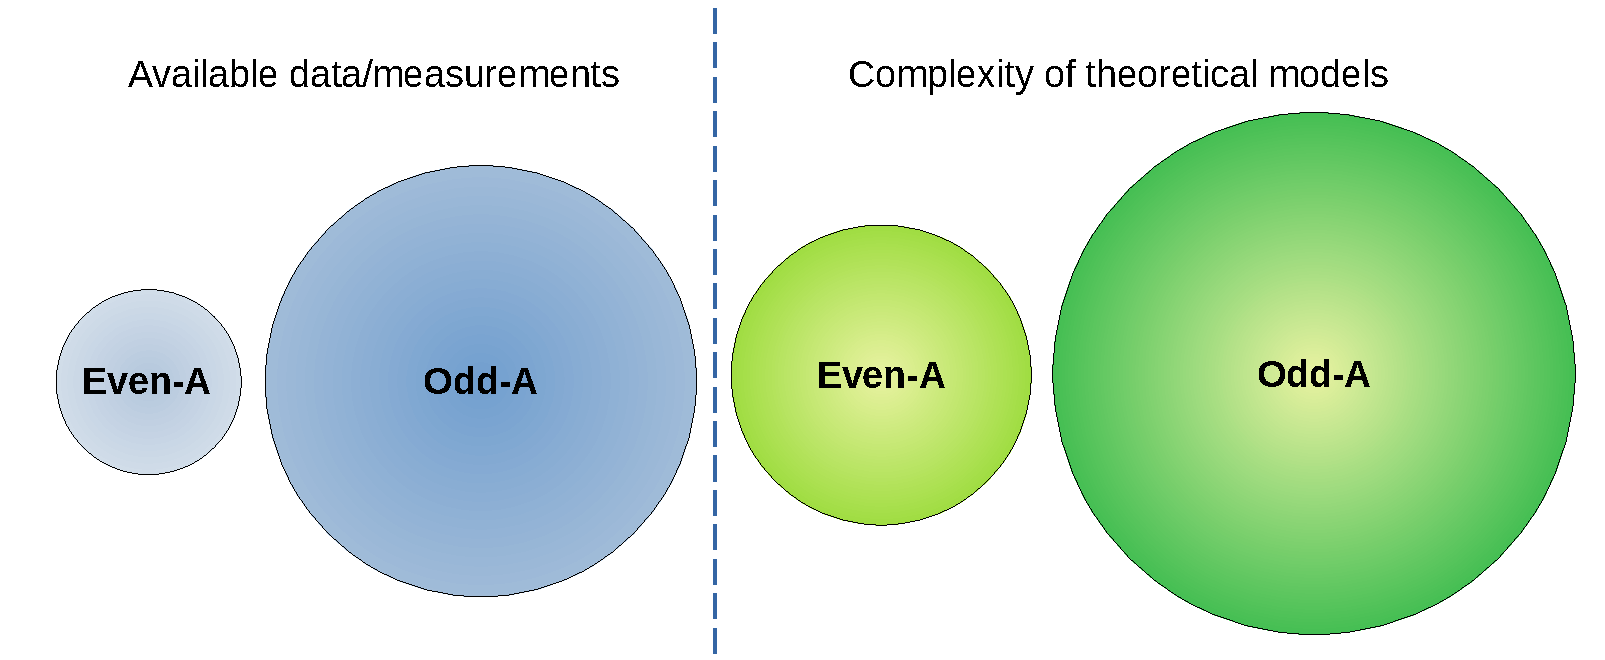
\includegraphics[width=0.99\textwidth]{figures/even-vs-odda.pdf}
	\end{figure}
\end{frame}

\section{Current status of nuclear "wobblers"}

\begin{frame}
    \frametitle{$A\approx100$}
    \textbf{Excitation energies} vs. \textbf{Wobbling Energies}:
	\begin{align}
		E_\text{wob}(I_\text{even})&=E_{I,n}-E_{I,0}\ ,\nonumber \\
		E_\text{wob}(I_\text{odd})&=E_{I,n}-\frac{1}{2}\left(E_{I-1,0}+E_{I+1,0}\right) \nonumber
	\end{align}
    \begin{figure}
        \centering
        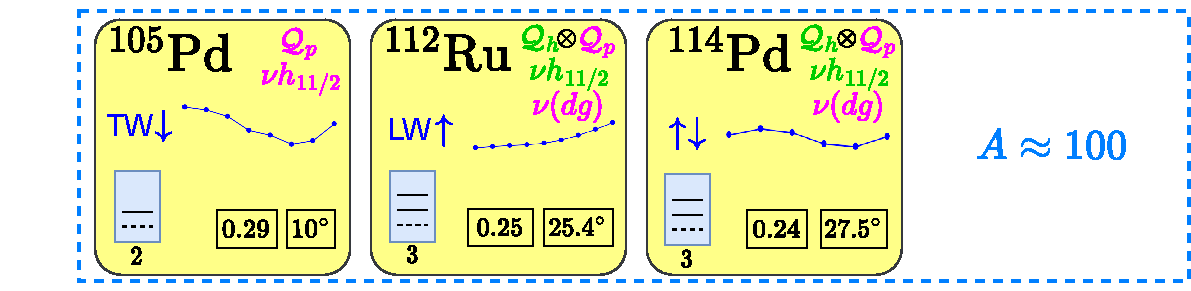
\includegraphics[width=0.99\textwidth]{figures/wobblers-chart-1.pdf}
        \caption{\textit{Experimentally confirmed wobblers, R Poenaru, 2023.}}
    \end{figure}
\end{frame}

\begin{frame}
    \frametitle{$A\approx130$}
    \begin{figure}
        \centering
        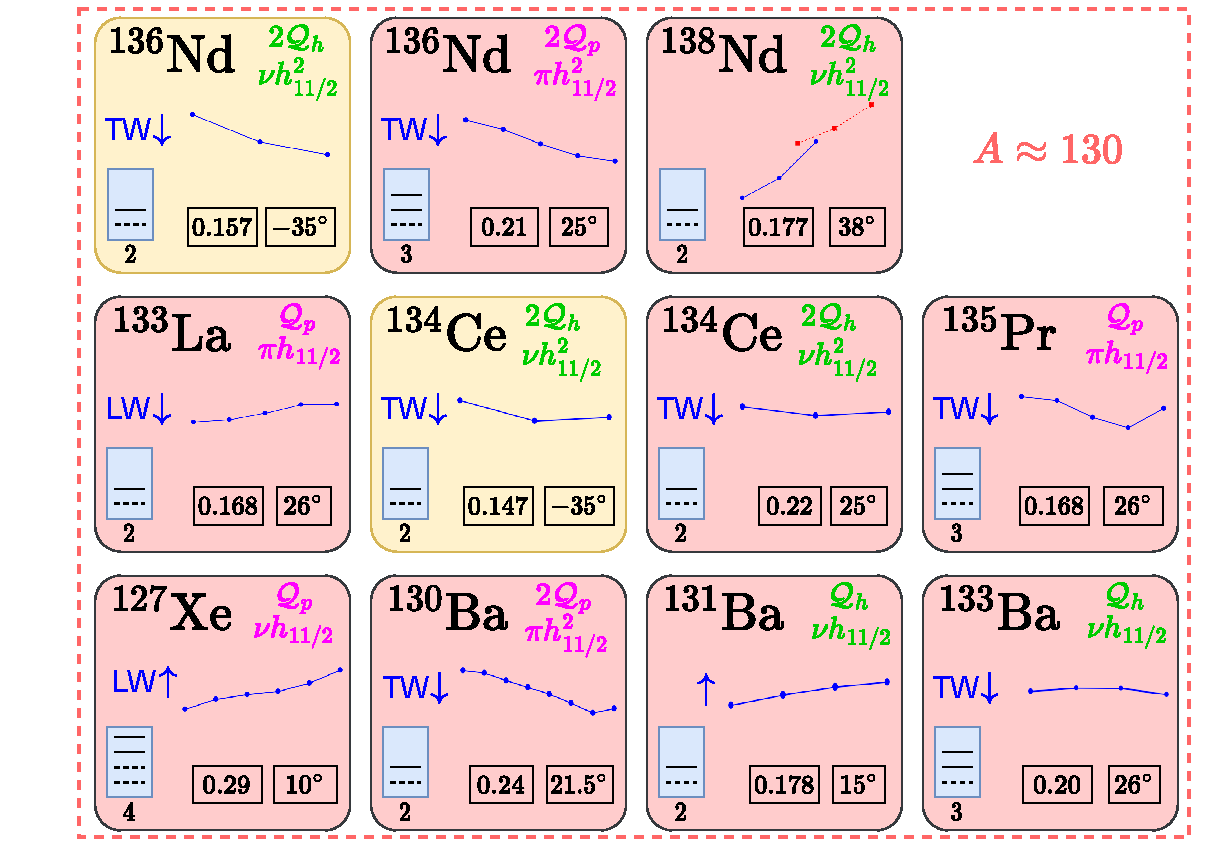
\includegraphics[width=0.75\textwidth]{figures/wobblers-chart-2.pdf}
        \caption{\textit{Experimentally confirmed wobblers, R Poenaru, 2023.}}
    \end{figure}
\end{frame}

\begin{frame}
    \frametitle{$A\approx160$}
    \begin{figure}
        \centering
        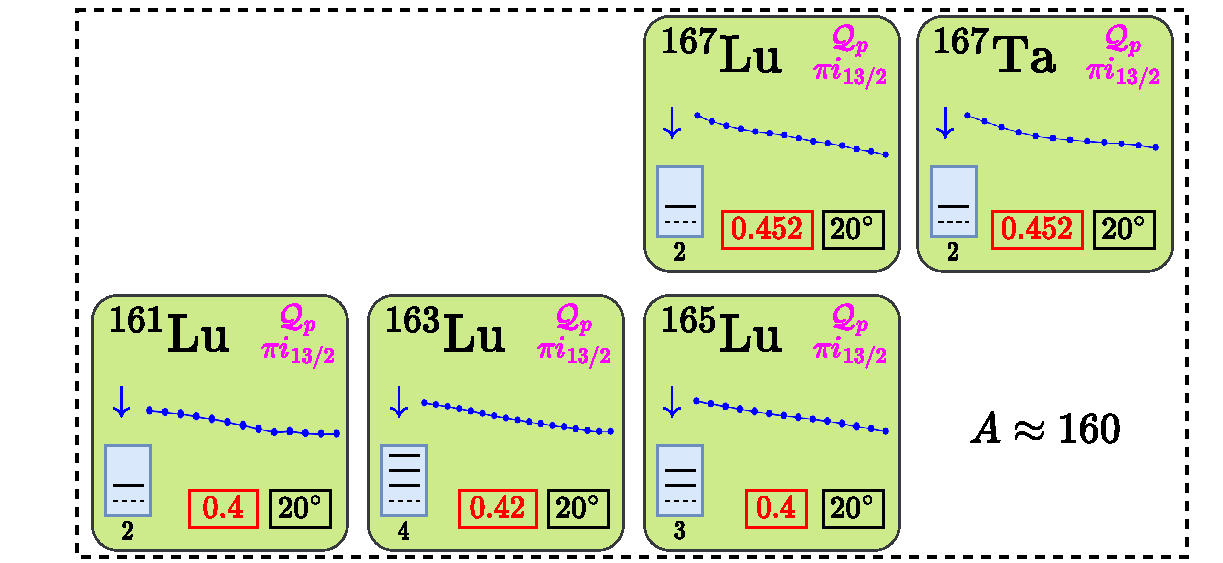
\includegraphics[width=0.99\textwidth]{figures/wobblers-chart-4.pdf}
        \caption{\textit{Experimentally confirmed wobblers, R Poenaru, 2023.}}
    \end{figure}
\end{frame}

\begin{frame}
    \frametitle{$A\approx180$}
    \begin{figure}
        \centering
        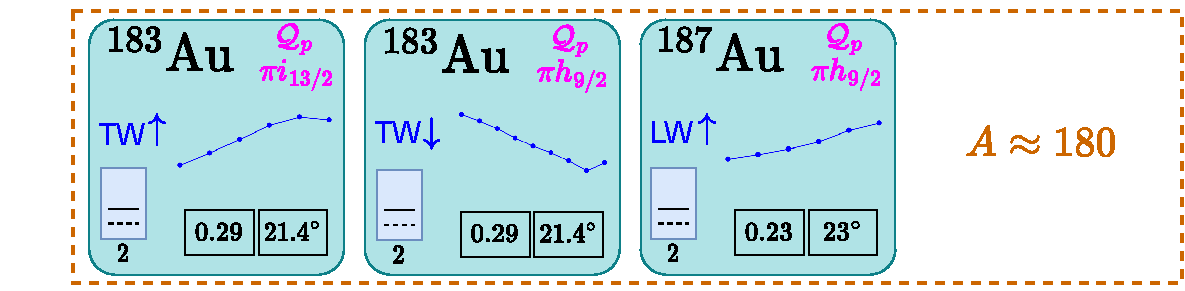
\includegraphics[width=0.99\textwidth]{figures/wobblers-chart-3.pdf}
        \caption{\textit{Experimentally confirmed wobblers, R Poenaru, 2023.}}
    \end{figure}
\end{frame}

\begin{frame}
    \frametitle{Wobbling Motion in $^{135}$Pr}
\end{frame}


\begin{frame}
	\begin{center}
		\bigskip\bigskip
		{\Huge Thank you for your attention!}
	\end{center}
\end{frame} 

\end{document}
